\documentclass[12pt, letterpaper]{article}

\usepackage[english]{babel} % Sets the language and regional settings for English documents
\usepackage[utf8]{inputenc} % Allows the use of UTF-8 characters in the document
\usepackage[T1]{fontenc} % Specifies t\subsubsection*{Forma canónica reducida}
\usepackage[margin=2cm]{geometry} % Sets the page margins
\usepackage{makeidx} % Enables the creation of indexes
% \usepackage{natbib} % Provides flexible bibliography support
\usepackage{url} % Allows the use of URLs
\usepackage{enumitem} % Customizes the appearance of lists
\usepackage{listings} % Provides syntax highlighting for code listings
\usepackage[dvipsnames]{xcolor} % Allows the use of colors
\usepackage{parskip} % Modifies paragraph spacing
\usepackage{graphicx} % Enables the inclusion of graphics
\usepackage{tikz} % Allows the creation of graphics and diagrams
\usepackage{float}
\usepackage{hyperref} % Enables the creation of hyperlinks
\usepackage{amsmath} % Provides additional math environments and commands
\usepackage{circuitikz} % Allows the creation of electrical circuits
\usepackage{adjustbox} % Adjusts the size of the circuit diagrams
\usepackage{tcolorbox}
\usepackage{diagbox} % Allows the use of diagonal boxes in table cells
\usepackage{colortbl} % Allows coloring of table cells
\hypersetup{
    colorlinks=true,
    linkcolor=blue,
    urlcolor=blue
}
\usepackage{breakurl} % permite que los links se rompan en varias líneas
\definecolor{mygray}{gray}{0.9}

\usetikzlibrary{shapes.geometric, positioning}

\lstset{
	language=SQL,
	basicstyle=\ttfamily\small,
	keywordstyle=\color{blue},
	commentstyle=\color[rgb]{0,0.5,0},
	stringstyle=\color{red},
	numbers=left,
	numberstyle=\tiny\color{gray},
	stepnumber=1,
	numbersep=10pt,
	backgroundcolor=\color{white},
	showspaces=false,
	showstringspaces=false,
	breaklines=true,
	frame=single,
	tabsize=2, captionpos=b, lineskip=-1pt,
	extendedchars=true,
	literate={á}{{\'a}}1 {é}{{\'e}}1 {í}{{\'i}}1 {ó}{{\'o}}1 {ú}{{\'u}}1 {Á}{{\'A}}1 {É}{{\'E}}1 {Í}{{\'I}}1 {Ó}{{\'O}}1 {Ú}{{\'U}}1 {ñ}{{\~n}}1 {Ñ}{{\~N}}1 {¿}{{\textquestiondown}}1 {¡}{{\textexclamdown}}1
}

% VHDL language configuration
\lstdefinelanguage{VHDL}{
	morekeywords={entity, architecture, signal, port, in, out, inout, begin, end, process, if, then, else, elsif, case, when, others, for, while, loop, wait, library, use, std_logic, std_logic_vector, integer, boolean, rising_edge, falling_edge, component, generic, map, downto, to, and, or, not, xor, nand, nor, xnor},
	morecomment=[l]{--},
	morestring=[b]",
	sensitive=false,
	alsoletter={_}
}

% VHDL listings style
\lstdefinestyle{vhdl}{
	language=VHDL,
	basicstyle=\ttfamily\small,
	keywordstyle=\color{blue}\bfseries,
	commentstyle=\color[rgb]{0,0.6,0}\itshape,
	stringstyle=\color{red},
	numbers=left,
	numberstyle=\tiny\color{gray},
	stepnumber=1,
	numbersep=10pt,
	backgroundcolor=\color{white},
	showspaces=false,
	showstringspaces=false,
	breaklines=true,
	frame=single,
	tabsize=2,
	captionpos=b,
	lineskip=-1pt,
	extendedchars=true
}

\graphicspath{ {./img/} } % Sets the path for the graphics

\newlist{biblio}{enumerate}{1}
\setlist[biblio,1]{label=[\arabic*]}

\makeindex

\begin{document}

\begin{titlepage}

	\begin{tikzpicture}[remember picture,overlay]
		\node[anchor=north west, inner sep=30] at (current page.north west) {
			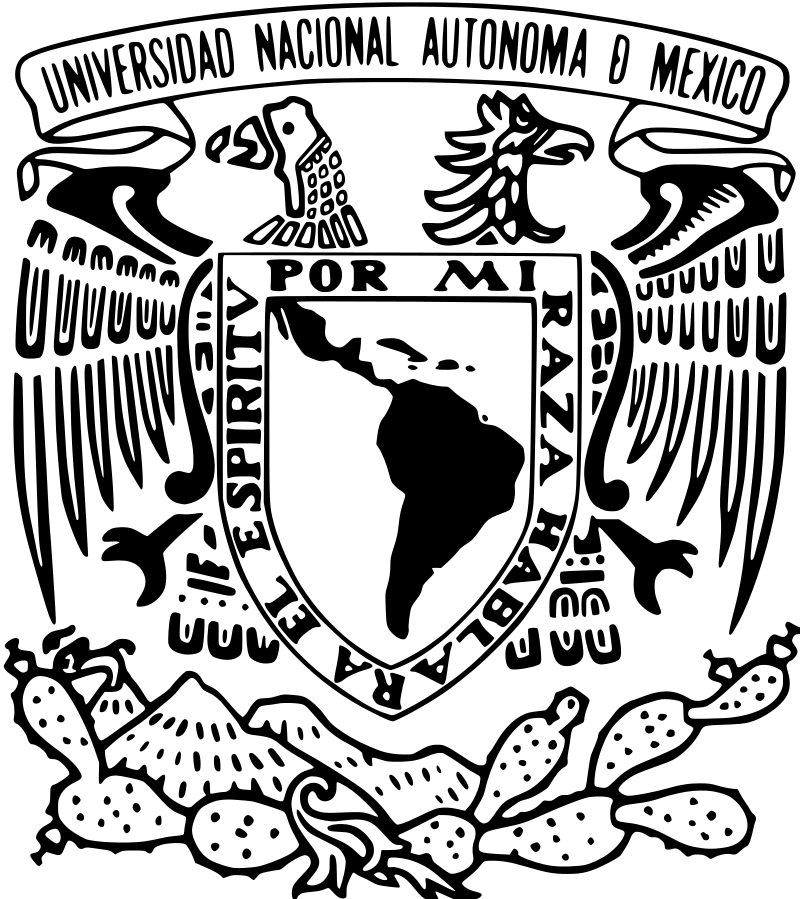
\includegraphics[width=4cm]{escudoUNAM.png}
		};

		\node[anchor=north east, inner sep=30] at (current page.north east) {
			
\includegraphics[width=4cm]{escudoFI.png}
		};
	\end{tikzpicture}

	\begin{center}
		\vspace*{3cm}

		\Huge
		\textbf{Práctica 4 - Escalamiento de Impedancia y Frecuencia}\\

		\vspace{2.5cm}

		\Huge
		\textbf{Facultad de Ingeniería}\\
		Circuitos Electrónicos\\
		\textbf{Ing. Martha Isela Torres Hernández} \\
		2026-1\\

		\vspace{2.5cm}

		\textbf{Grupo:} 4\\

		\vspace{2.5cm}

		\Huge
		\textbf{Integrantes Brigada 6:}\\
		Ugartechea González Luis Antonio\\
		Tepal Briseño Hansel Yael\\
		\textbf{Fecha de entrega:} 28 de octubre del 2025\\
		\vspace{2.5cm}
	\end{center}
\end{titlepage}

\section{objetivos}

\begin{itemize}
	\item Presentación de los teoremas de escalamiento de impedancia y de frecuencia.
	\item Familiarizar al alumno con la aplicación práctica de dichos teoremas.
	\item Apreciar la importancia de tales teoremas en el diseño de filtros eléctricos.
\end{itemize}

\section{Introducción}

El escalamiento de impedancia y el escalamiento de frecuencia son teoremas fundamentales utilizados en el análisis y diseño de circuitos electrónicos. Estos métodos proporcionan una técnica sistemática para modificar los valores de los componentes de un circuito (resistencias, inductores y capacitores) con el fin de ajustar sus características operativas. El escalamiento de impedancia permite cambiar los niveles de impedancia de un circuito sin alterar su respuesta en frecuencia, mientras que el escalamiento de frecuencia permite desplazar la respuesta en frecuencia del circuito a una nueva banda de operación sin cambiar la forma de dicha respuesta.

La aplicación práctica de estos teoremas es de gran importancia, particularmente en el diseño de filtros eléctricos. A menudo, los diseños de filtros comienzan a partir de un prototipo normalizado (por ejemplo, con una frecuencia de corte de 1 rad/s y resistencias de 1 ohm). Mediante el uso de los teoremas de escalamiento, este diseño prototipo puede transformarse eficientemente para cumplir con los requisitos específicos de frecuencia de corte e impedancia de una aplicación en el mundo real, facilitando enormemente el proceso de diseño.

\section{Desarrollo}

\subsection{Cálculos previos con el circuito original}

\begin{figure}[H]
	\centering
	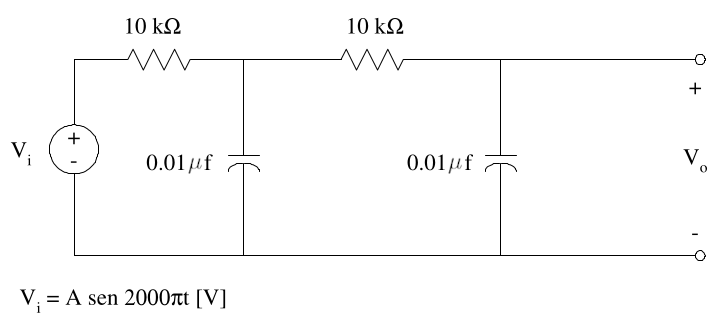
\includegraphics[width=0.8\textwidth]{circuito.png}
	\caption{Circuito RC}
	\label{fig:circuito}
\end{figure}

\subsubsection*{Medición del desfase entre \(V_o\) y \(V_i\)}

Simulando el circuito de la figura \ref{fig:circuito} en Multisim:

\begin{figure}[H]
	\centering
	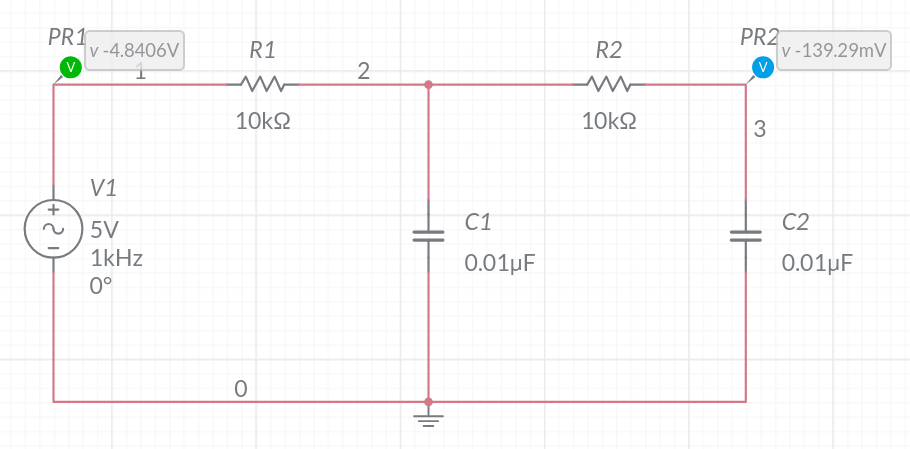
\includegraphics[width=0.9\textwidth]{original_circuito.png}
	\caption{Circuito original en multisim}
	\label{fig:original_circuito}
\end{figure}

Se obtiene la siguiente gráfica de respuesta en frecuencia:

\begin{figure}[H]
	\centering
	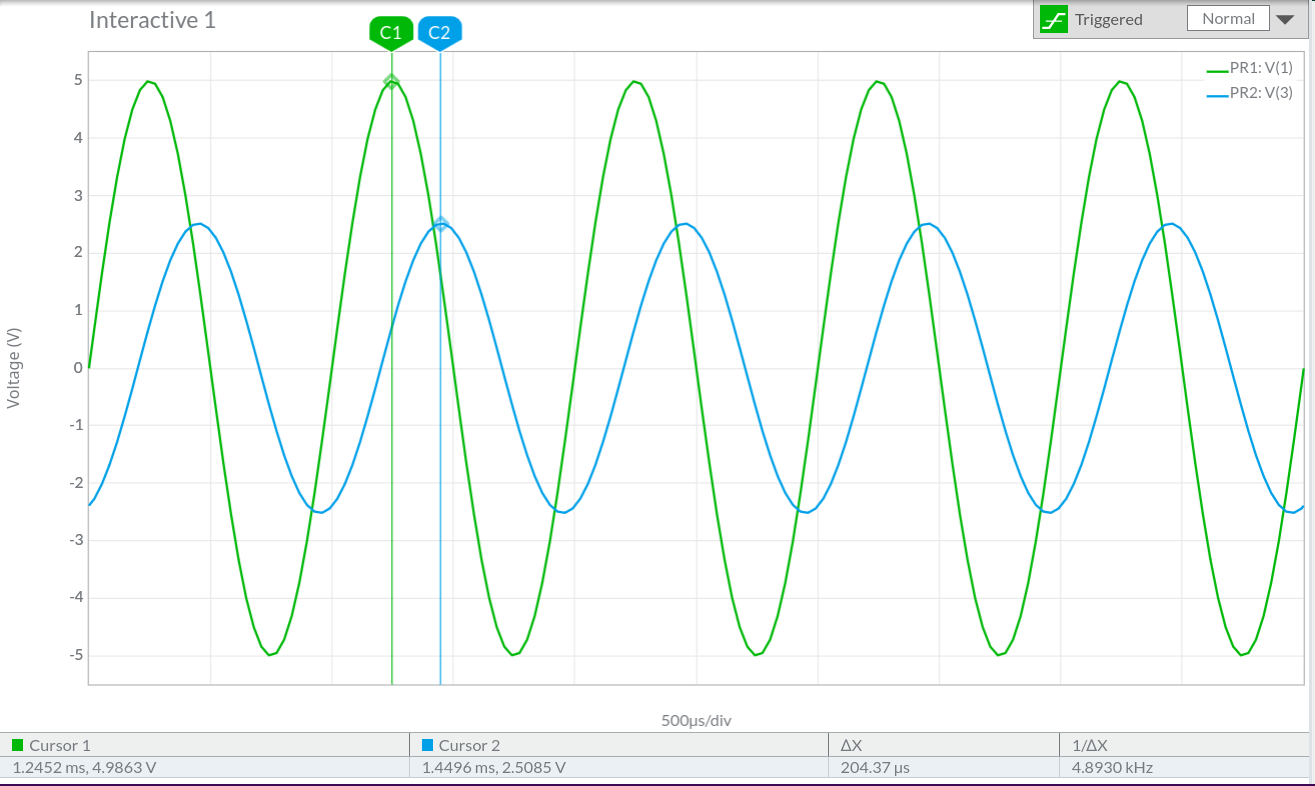
\includegraphics[width=0.9\textwidth]{original_grafica.png}
	\caption{Respuesta en frecuencia del circuito original}
	\label{fig:original_grafica}
\end{figure}

Con esto podemos observar que el desfase entre \(V_o\) y \(V_i\) es de \(204.37 ms\). Con este dado y con la referencia de que el periodo de entrada medido es de \(T = 1.0029 ms\), podemos calcular el ángulo de desfase \(\phi\) con la regla de tres:

\[\phi = \frac{204.37 ms \cdot 360^{\circ}}{1.0029 ms}\]

\textbf{Resultado:}

\begin{tcolorbox}[colback=mygray, colframe=LimeGreen, boxrule=0.7pt, arc=2pt, boxsep=1pt, left=2pt, right=2pt, top=2pt, bottom=2pt, title=Ángulo de desfase]
\(\phi = 73.36^{\circ}\)
\end{tcolorbox}

\subsubsection*{Magnitud de \(V_o\) respecto a \(V_i\)}

\(|H(j2000\pi)| = \frac{V_o}{V_i} = \frac{2.5085}{4.9863 V}\)

\textbf{Resultado:}

\begin{tcolorbox}[colback=mygray, colframe=LimeGreen, boxrule=0.7pt, arc=2pt, boxsep=1pt, left=2pt, right=2pt, top=2pt, bottom=2pt, title=Magnitud de \(H(j2000\pi)\)]
\(|H(j2000\pi)| = 0.503\)
\end{tcolorbox}

\section{Experimento 1 (Escalamiento de Impedancia)}

\begin{figure}[H]
	\centering
	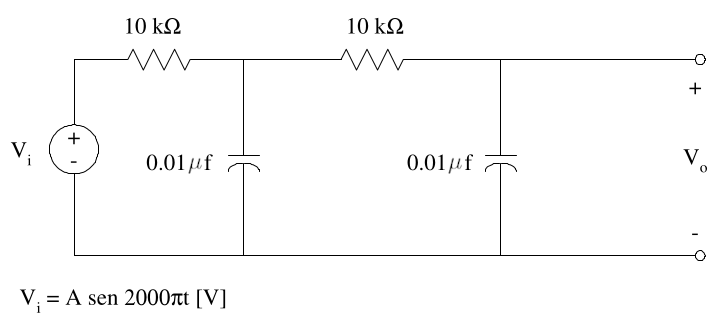
\includegraphics[width=0.8\textwidth]{circuito.png}
	\caption{Circuito RC}
	\label{fig:circuito_impedancia}
\end{figure}

Determinar el valor de los capacitores si cambiamos las resistencias a \(R = 1 k \Omega\).

\subsection*{Obtención de k\_m}

\[k_m = \frac{R_{q}}{R_{t}} = \frac{1 k\Omega}{10 k\Omega} = \frac{1}{10}\]

\begin{figure}[H]
	\centering
	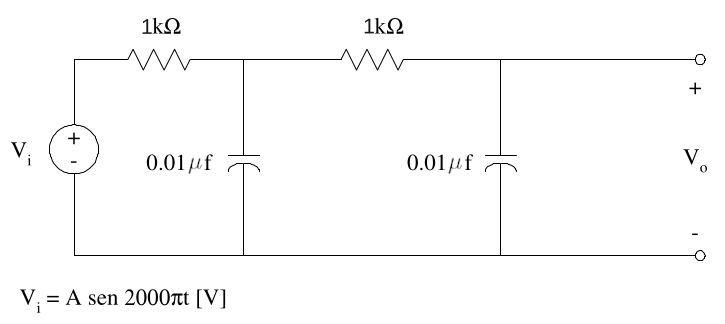
\includegraphics[width=0.8\textwidth]{circuito_e1_p1.png}
	\caption{Circuito RC con nueva resistencia}
	\label{fig:circuito_e1_p1}
\end{figure}

\subsection*{Cálculo del nuevo valor del capacitor}

Con respecto a la figura \ref{fig:circuito_e1_p1}, el valor del los capacitores originales es \(C_{t} = 0.01 \mu F\). El nuevo valor del capacitor \(C_{q}\) se obtiene con la siguiente fórmula:

\[C_{q} = \frac{C_{t}}{k_m}\]

Sustituyendo los valores:

\[C_{q} = \frac{0.01 \mu F}{\frac{1}{10}} = 0.1 \mu F\]

Dejándonos con el siguiente resultado:

\begin{figure}[H]
	\centering
	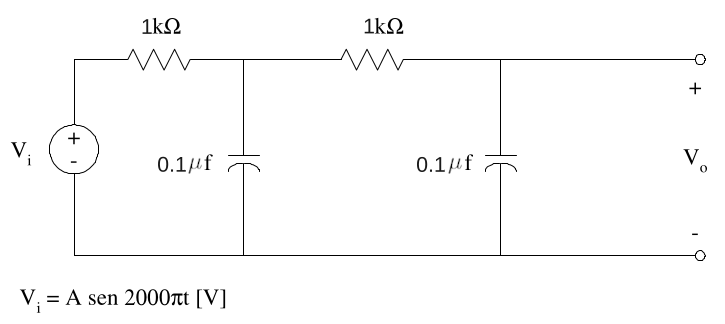
\includegraphics[width=0.8\textwidth]{circuito_e1_p2.png}
	\caption{Circuito RC con nuevo capacitor}
	\label{fig:circuito_e1_p2}
\end{figure}

\subsection*{Simulación en Multisim}

Simulando el circuito de la figura \ref{fig:circuito_e1_p2} en Multisim:

\begin{figure}[H]
	\centering
	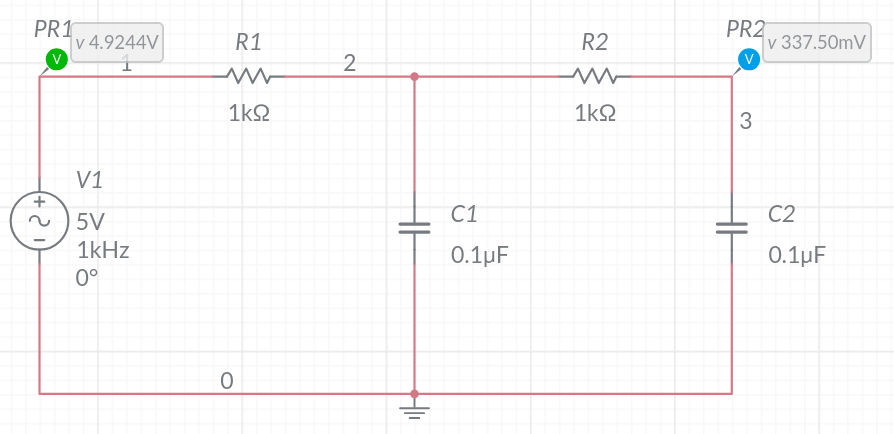
\includegraphics[width=0.9\textwidth]{ejercicio1_circuito.png}
	\caption{Circuito escalado en multisim}
	\label{fig:e1_circuito}
\end{figure}

Se obtiene la siguiente gráfica de respuesta en frecuencia:

\begin{figure}[H]
	\centering
	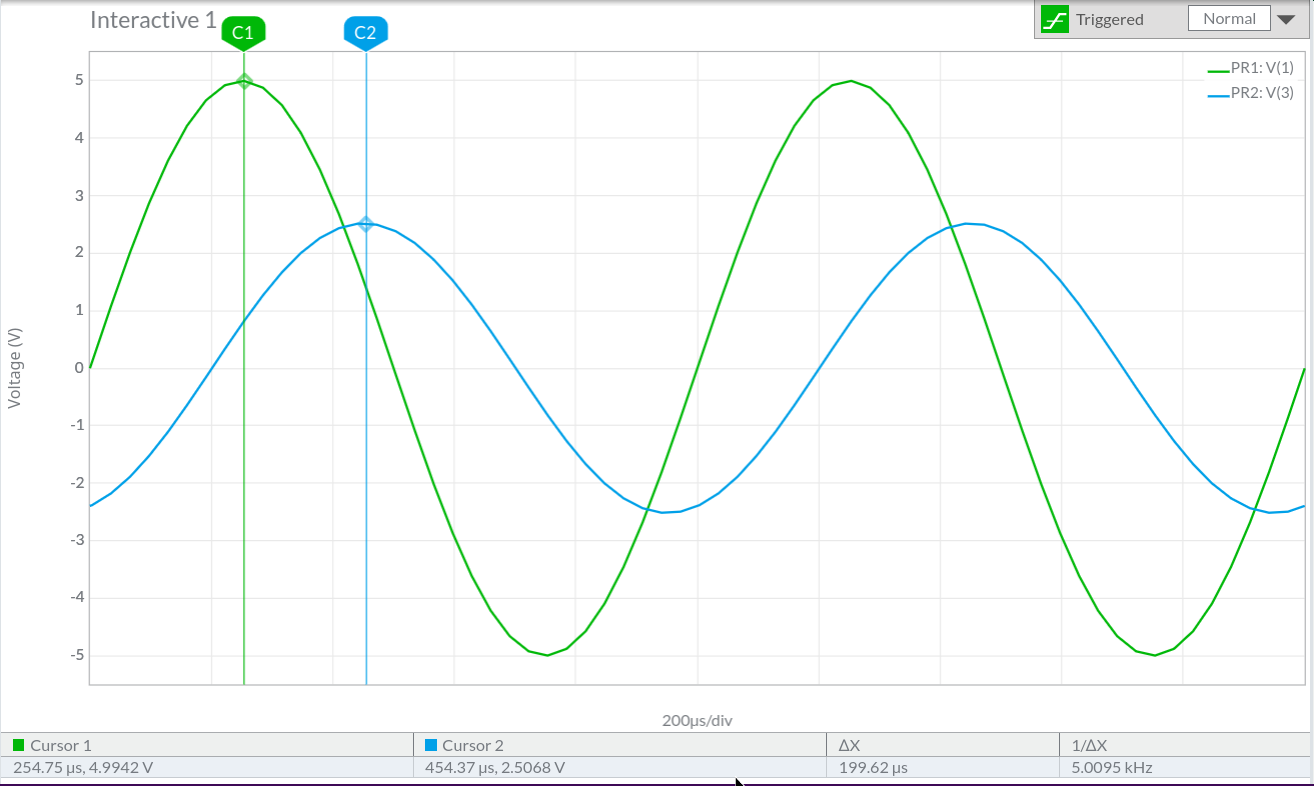
\includegraphics[width=0.9\textwidth]{ejercicio1_grafica.png}
	\caption{Respuesta en frecuencia del circuito escalado}
	\label{fig:e1_grafica}
\end{figure}

\subsubsection*{Medición del desfase entre \(V_o\) y \(V_i\)}

Con esto podemos observar que el desfase entre \(V_o\) y \(V_i\) es de \(199.62 ms\). Con este dado y con la referencia de que el periodo de entrada medido es de \(T = 1 ms\), podemos calcular el ángulo de desfase \(\phi\) con la regla de tres:

\[\phi = \frac{199.62 ms \cdot 360^{\circ}}{1 ms}\]

\textbf{Resultado:}

\begin{tcolorbox}[colback=mygray, colframe=LimeGreen, boxrule=0.7pt, arc=2pt, boxsep=1pt, left=2pt, right=2pt, top=2pt, bottom=2pt, title=Ángulo de desfase]
\(\phi = 71.55^{\circ}\)
\end{tcolorbox}

\subsubsection*{Magnitud de \(V_o\) respecto a \(V_i\)}

\(|H(j2000\pi)| = \frac{V_o}{V_i} = \frac{2.5068 V}{4.9942 V}\)

\textbf{Resultado:}

\begin{tcolorbox}[colback=mygray, colframe=LimeGreen, boxrule=0.7pt, arc=2pt, boxsep=1pt, left=2pt, right=2pt, top=2pt, bottom=2pt, title=Magnitud de \(H(j2000\pi)\)]
\(|H(j2000\pi)| = 0.5019\)
\end{tcolorbox}

\section{Experimento 2 (Escalamiento de Frecuencia)}

\begin{figure}[H]
	\centering
	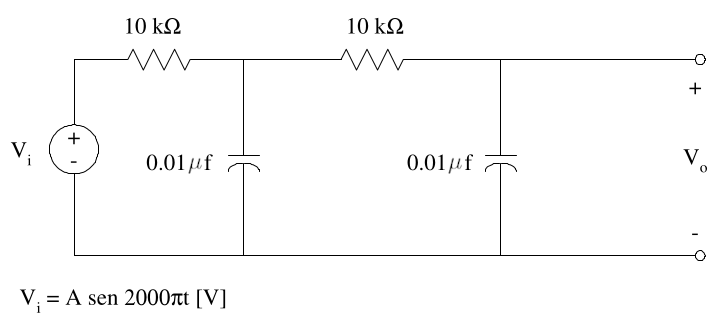
\includegraphics[width=0.8\textwidth]{circuito.png}
	\caption{Circuito RC}
	\label{fig:circuito_frecuencia}
\end{figure}

Determinar los valores de los capacitores cuando \(V_i = 5 sen(1000 \pi t)\).

\subsection*{Obtención de k\_f}

\[k_f = \frac{\omega_{t}}{\omega_{1}} = \frac{2000 \pi}{1000 \pi} = 2\]

\begin{figure}[H]
	\centering
	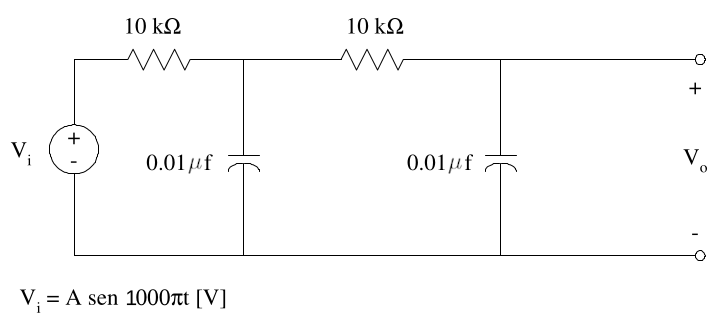
\includegraphics[width=0.8\textwidth]{circuito_e2_p1.png}
	\caption{Circuito RC con nueva frecuencia}
	\label{fig:circuito_e2_p1}
\end{figure}

\subsection*{Cálculo del nuevo valor del capacitor}

Con respecto a la figura \ref{fig:circuito_e2_p1}, el valor del los capacitores originales es \(C_{t} = 0.01 \mu F\). El nuevo valor del capacitor \(C_{q}\) se obtiene con la siguiente fórmula:

\[C_{q} = C_{t} \cdot k_f\]

Sustituyendo los valores:

\[C_{q} = 0.01 \mu F \cdot 2 = 0.02 \mu F\]

Dejándonos con el siguiente resultado:

\begin{figure}[H]
	\centering
	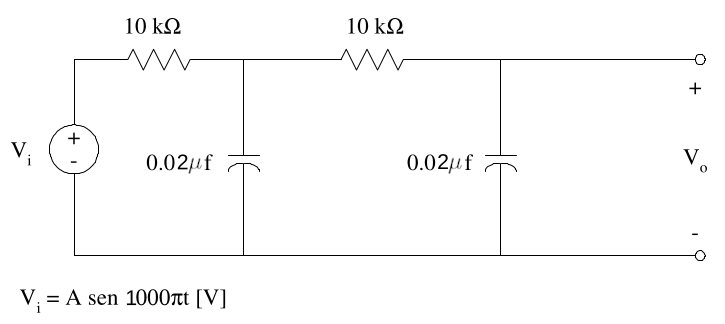
\includegraphics[width=0.8\textwidth]{circuito_e2_p2.png}
	\caption{Circuito RC con nuevo capacitor}
	\label{fig:circuito_e2_p2}
\end{figure}

\subsection*{Simulación en Multisim}

Simulando el circuito de la figura \ref{fig:circuito_e2_p2} en Multisim:

\begin{figure}[H]
	\centering
	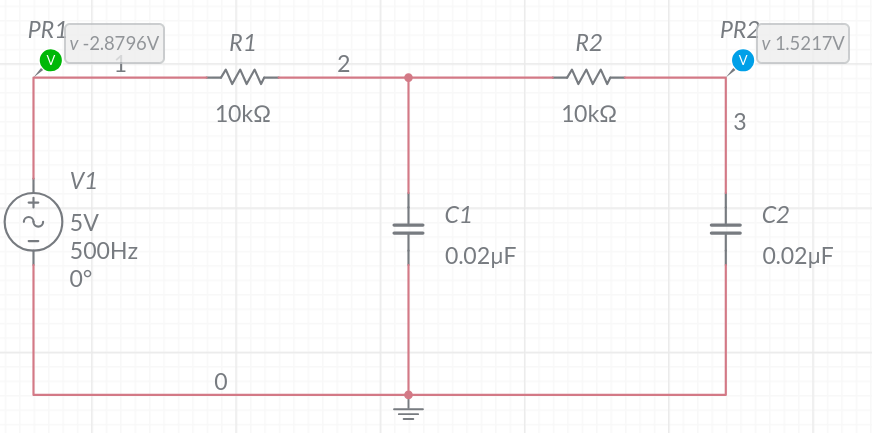
\includegraphics[width=0.9\textwidth]{ejercicio2_circuito.png}
	\caption{Circuito escalado en multisim}
	\label{fig:e2_circuito}
\end{figure}

Se obtiene la siguiente gráfica de respuesta en frecuencia:

\begin{figure}[H]
	\centering
	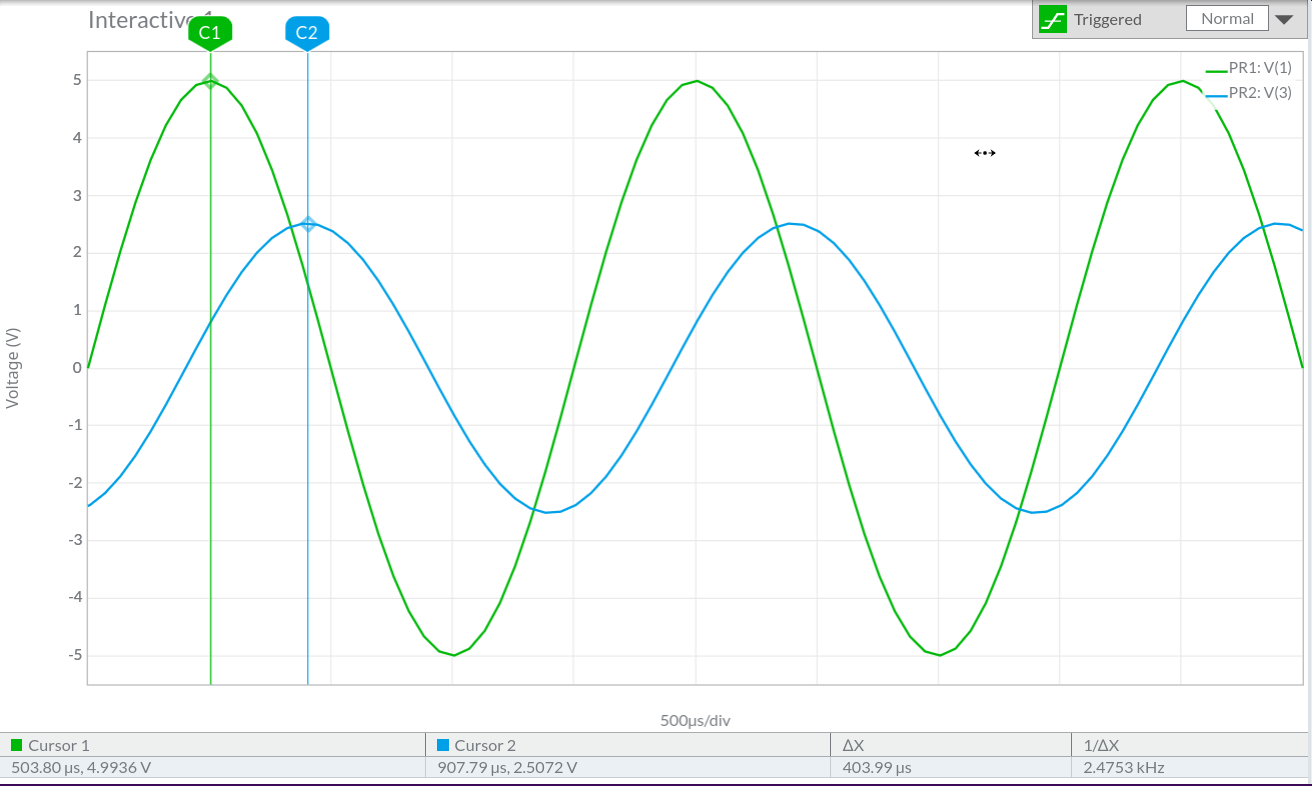
\includegraphics[width=0.9\textwidth]{ejercicio2_grafica.png}
	\caption{Respuesta en frecuencia del circuito escalado}
	\label{fig:e2_grafica}
\end{figure}

\subsubsection*{Medición del desfase entre \(V_o\) y \(V_i\)}

Con esto podemos observar que el desfase entre \(V_o\) y \(V_i\) es de \(403.99 ms\). Con este dado y con la referencia de que el periodo de entrada medido es de \(T = 1.9962 ms\), podemos calcular el ángulo de desfase \(\phi\) con la regla de tres:

\[\phi = \frac{403.99 ms \cdot 360^{\circ}}{1.9962 ms}\]

\textbf{Resultado:}

\begin{tcolorbox}[colback=mygray, colframe=LimeGreen, boxrule=0.7pt, arc=2pt, boxsep=1pt, left=2pt, right=2pt, top=2pt, bottom=2pt, title=Ángulo de desfase]
\(\phi = 72.85^{\circ}\)
\end{tcolorbox}

\subsubsection*{Magnitud de \(V_o\) respecto a \(V_i\)}

\(|H(j1000\pi)| = \frac{V_o}{V_i} = \frac{2.5072 V}{4.9936 V}\)

\textbf{Resultado:}
\begin{tcolorbox}[colback=mygray, colframe=LimeGreen, boxrule=0.7pt, arc=2pt, boxsep=1pt, left=2pt, right=2pt, top=2pt, bottom=2pt, title=Magnitud de \(H(j1000\pi)\)]
\(|H(j1000\pi)| = 0.5021\)
\end{tcolorbox}

\section{Experimento 3 (Escalamiento de Impedancia y Frecuencia)}

\begin{figure}[H]
	\centering
	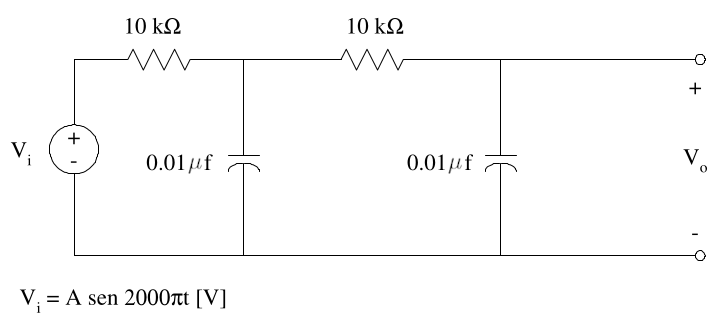
\includegraphics[width=0.8\textwidth]{circuito.png}
	\caption{Circuito RC}
	\label{fig:circuito_impedancia_frecuencia}
\end{figure}

Si \(R = 1k \Omega\), cuanto deben valer los capacitores para que \(V_i = 5 sen(4000 \pi t)\).

\subsection*{Obtención de k\_m y k\_f}

Para escalamiento de impedancia:

\[k_m = \frac{R_{q}}{R_{t}} = \frac{1 k\Omega}{10 k\Omega} = \frac{1}{10}\]

Para escalamiento de frecuencia:

\[k_f = \frac{\omega_{t}}{\omega_{1}} = \frac{2000 \pi}{4000 \pi} = \frac{1}{2}\]

\begin{figure}[H]
	\centering
	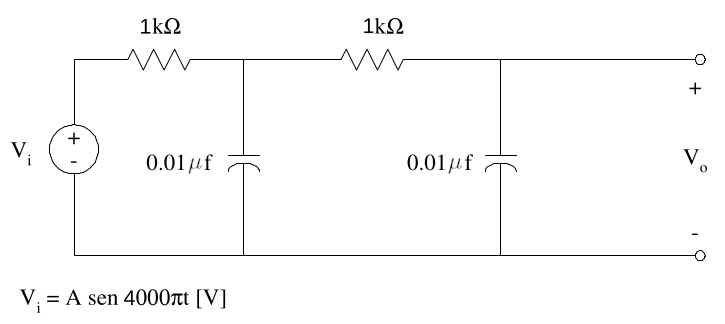
\includegraphics[width=0.8\textwidth]{circuito_e3_p1.png}
	\caption{Circuito RC con nueva resistencia y frecuencia}
	\label{fig:circuito_e3_p1}
\end{figure}

\subsection*{Cálculo del nuevo valor del capacitor en impedancia}

\[C_{q1} = \frac{C_{t}}{k_m}\]

Sustituyendo los valores:

\[C_{q1} = \frac{0.01 \mu F}{\frac{1}{10}} = 0.1 \mu F\]

\subsection*{Cálculo del nuevo valor del capacitor en frecuencia}

\[C_{q2} = C_{q1} \cdot k_f\]

Sustituyendo los valores:

\[C_{q2} = 0.1 \mu F \cdot \frac{1}{2} = 0.05 \mu F\]

Dejándonos con el siguiente resultado:

\begin{figure}[H]
	\centering
	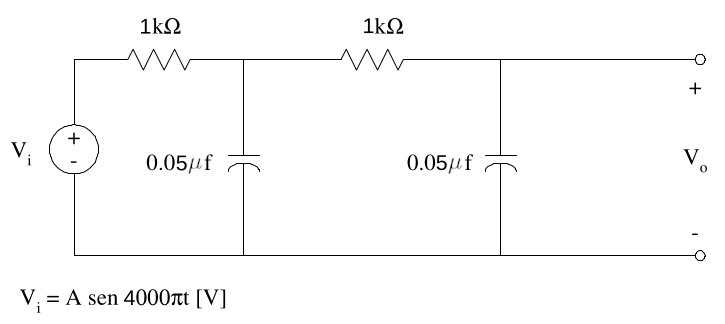
\includegraphics[width=0.8\textwidth]{circuito_e3_p2.png}
	\caption{Circuito RC con nuevo capacitor}
	\label{fig:circuito_e3_p2}
\end{figure}

\subsection*{Simulación en Multisim}

Simulando el circuito de la figura \ref{fig:circuito_e3_p2} en Multisim:

\begin{figure}[H]
	\centering
	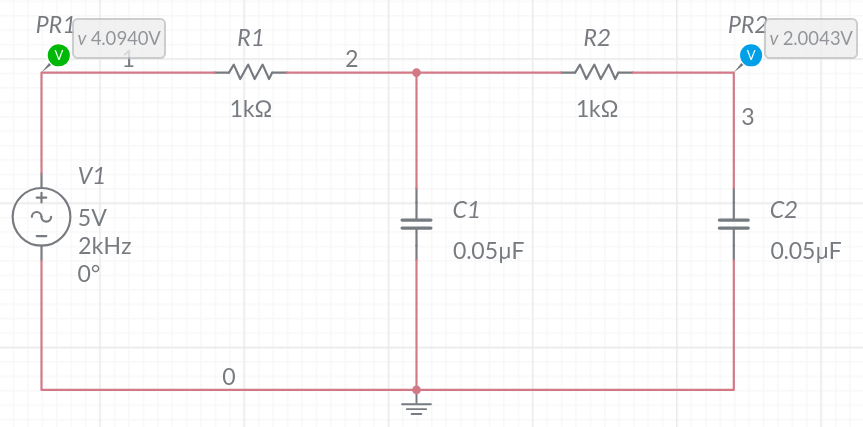
\includegraphics[width=0.9\textwidth]{ejercicio3_circuito.png}
	\caption{Circuito escalado en multisim}
	\label{fig:e3_circuito}
\end{figure}

Se obtiene la siguiente gráfica de respuesta en frecuencia:

\begin{figure}[H]
	\centering
	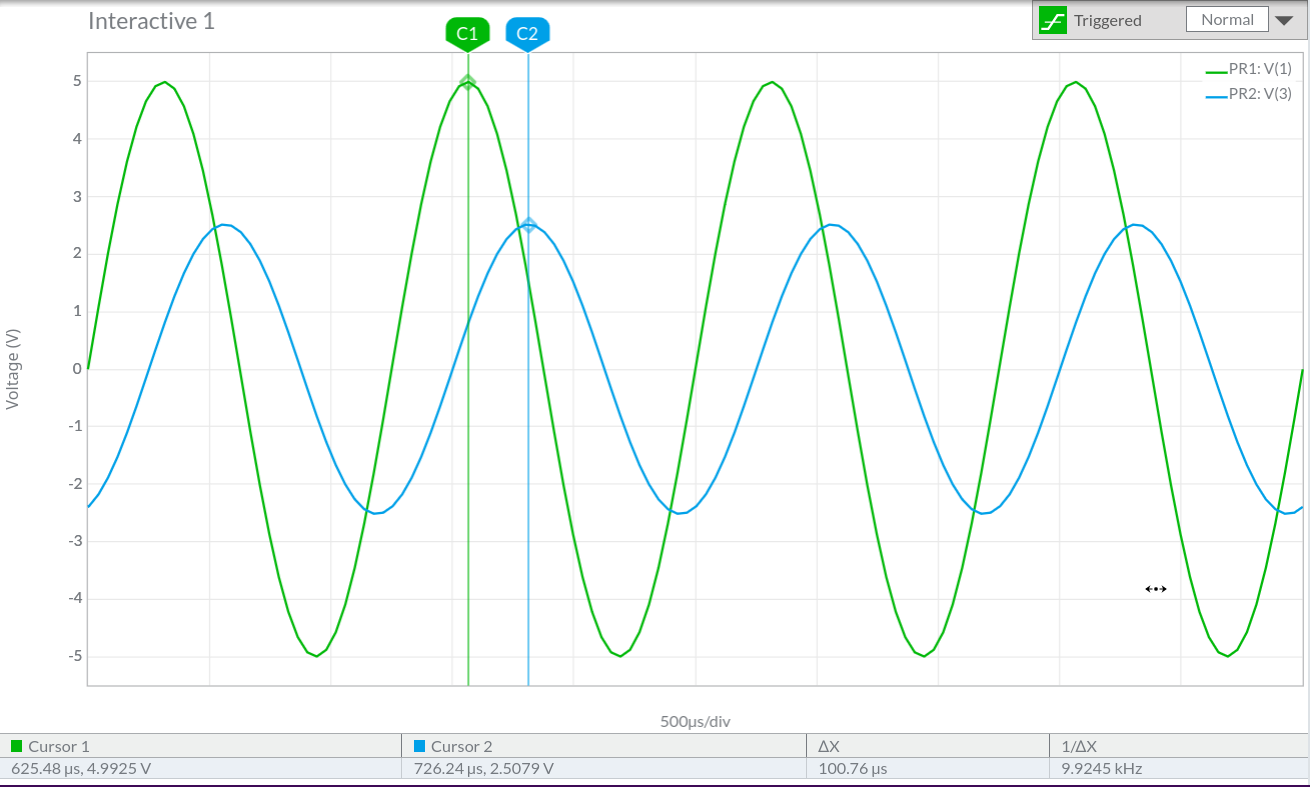
\includegraphics[width=0.9\textwidth]{ejercicio3_grafica.png}
	\caption{Respuesta en frecuencia del circuito escalado}
	\label{fig:e3_grafica}
\end{figure}

\subsubsection*{Medición del desfase entre \(V_o\) y \(V_i\)}

Con esto podemos observar que el desfase entre \(V_o\) y \(V_i\) es de \(100.76 ms\). Con este dado y con la referencia de que el periodo de entrada medido es de \(501.9 ms\), podemos calcular el ángulo de desfase \(\phi\) con la regla de tres:

\[\phi = \frac{100.76 ms \cdot 360^{\circ}}{501.9 ms}\]

\textbf{Resultado:}
\begin{tcolorbox}[colback=mygray, colframe=LimeGreen, boxrule=0.7pt, arc=2pt, boxsep=1pt, left=2pt, right=2pt, top=2pt, bottom=2pt, title=Ángulo de desfase]
\(\phi = 72.27^{\circ}\)
\end{tcolorbox}

\subsubsection*{Magnitud de \(V_o\) respecto a \(V_i\)}

\(|H(j4000\pi)| = \frac{V_o}{V_i} = \frac{2.5079 V}{4.9925 V}\)

\textbf{Resultado:}
\begin{tcolorbox}[colback=mygray, colframe=LimeGreen, boxrule=0.7pt, arc=2pt, boxsep=1pt, left=2pt, right=2pt, top=2pt, bottom=2pt, title=Magnitud de \(H(j4000\pi)\)]
\(|H(j4000\pi)| = 0.5024\)
\end{tcolorbox}

\section{Error Porcentual entre el circuito original y los escalados}

\subsection*{Experimento 1}

\subsubsection*{Ángulo de desfase}

\[\text{Error porcentual} = \left|\frac{73.36 - 71.55}{73.36}\right| \times 100 = 2.46\%\]

\subsubsection*{Magnitud de \(H(j2000\pi)\)}

\[\text{Error porcentual} = \left|\frac{0.503 - 0.5019}{0.503}\right| \times 100 = 0.21\%\]

\subsection*{Experimento 2}

\subsubsection*{Ángulo de desfase}

\[\text{Error porcentual} = \left|\frac{73.36 - 72.85}{73.36}\right| \times 100 = 0.69\%\]

\subsubsection*{Magnitud de \(H(j4000\pi)\)}

\[\text{Error porcentual} = \left|\frac{0.503 - 0.5021}{0.503}\right| \times 100 = 0.17\%\]

\subsection*{Experimento 3}

\subsubsection*{Ángulo de desfase}

\[\text{Error porcentual} = \left|\frac{73.36 - 72.27}{73.36}\right| \times 100 = 1.48\%\]

\subsubsection*{Magnitud de \(H(j2000\pi)\)}

\[\text{Error porcentual} = \left|\frac{0.503 - 0.5024}{0.503}\right| \times 100 = 0.12\%\]

\subsection*{Tabla comparativa}

\begin{table}[H]
	\centering
	\begin{tabular}{|c|c|c|c|}
		\hline
		\textbf{Experimento} & \textbf{Parámetro} & \textbf{Valor Escalado} & \textbf{Error Porcentual} \\
		\hline
		0 & Ángulo de desfase & \(73.36^{\circ}\) & - \\
		\hline
		0 & Magnitud de \(H(j2000\pi)\) & \(0.503\) & - \\
		\hline
		1 & Ángulo de desfase & \(71.55^{\circ}\) & \(2.46\%\) \\
		\hline
		1 & Magnitud de \(H(j2000\pi)\) & \(0.5019\) & \(0.21\%\) \\
		\hline
		2 & Ángulo de desfase & \(72.85^{\circ}\) & \(0.69\%\) \\
		\hline
		2 & Magnitud de \(H(j1000\pi)\) & \(0.5021\) & \(0.17\%\) \\
		\hline
		3 & Ángulo de desfase & \(72.27^{\circ}\) & \(1.48\%\) \\
		\hline
		3 & Magnitud de \(H(j4000\pi)\) & \(0.5024\) & \(0.12\%\) \\
		\hline
	\end{tabular}
	\caption{Comparativa de resultados entre el circuito original y los escalados}
	\label{tab:comparativa_resultados}
\end{table}

\section{Conclusiones}

\subsection*{Hansel Yael Tepal Briseño}

Como se observa no hubo realmente una diferencia significativa entre el circuito original y los escalados, la diferencia fue menor al 3\%, validando la efectividad de los teoremas de escalamiento. El escalamiento de impedancia demostró ser útil para adaptar circuitos a diferentes niveles de potencia y compatibilidad con otros componentes del sistema, mientras que el escalamiento de frecuencia permite ajustar el circuito en base a la frecuencia de operación deseada. La combinación de ambos teoremas demuestra que es completamente flexible el uso separa y en conjunto, facilitando el diseño de circuitos electrónicos en diversas aplicaciones prácticas.

\subsection*{Luis Antonio Ugartechea González}

A pesar de la práctica simulada se comprobaron los teoremas de escalamiento de impedancia y frecuencia mediante la simulación de circuitos RC. Los resultados obtenidos demuestran que el escalamiento de impedancia permite modificar los valores de resistencia manteniendo la respuesta en frecuencia del circuito prácticamente inalterada, como se observó en el experimento 1 donde el error en el ángulo de desfase fue únicamente del 2.46\%. Asimismo, el escalamiento de frecuencia mostró su efectividad para desplazar la respuesta del circuito a diferentes bandas de frecuencia sin alterar significativamente la magnitud de la función de transferencia, evidenciado por errores menores al 1\% en todos los experimentos.

% \renewcommand{\refname}{}
% \begin{thebibliography}{9}
%    \bibitem{} Dr. E. García, \textit{"Diseño Digital VLSI Repaso DDM"}, presentado en el curso de Diseño Digital VLSI, Ciudad de México, 2025.
% \end{thebibliography}

\end{document}
